% !TeX root = RJwrapper.tex
\title{\pkg{dycdtools}: an R Package for Assisting Calibration and Visualising Outputs of an Aquatic Ecosystem Model}
\author{by Songyan Yu, Christopher G. McBride, Marieke A. Frassl, Matthew R. Hipsey and David P. Hamilton}

\maketitle

\abstract{
The high complexity of aquatic ecosystem models (AEMs) necessitates a large number of parameters that need calibration, and visualisation of their multifaceted and multi-layered simulation results is necessary for effective communication. Here we present an R package “dycdtools” that contains calibration and post-processing tools for a widely applied aquatic ecosystem model (DYRESM-CAEDYM). The calibration assistant function within the package automatically tests a large number of combinations of parameter values and returns corresponding values for goodness-of-fit, allowing users to narrow parameter ranges or optimise parameter values. The post-processing functions enable users to visualise modelling outputs in four ways: as contours, profiles, time series, and scatterplots. The “dycdtools” package is the first open-source calibration and post-processing tool for DYRESM-CAEDYM, and can also be adjusted for other AEMs with a similar structure. This package is useful to reduce the calibration burden for users and to effectively communicate model results with a broader community.}

\section{Introduction}

Aquatic ecosystem models are important tools to understand the structure and function of aquatic ecosystems, fill observation gaps, and support scientific management of water quality of inland waters \citep{jakeman2006ten}. Processed-based aquatic ecosystem models represent the major physical, chemical and biological processes as a series of mathematical equations, offering opportunities for exploratory or predictive management applications \citep{frassl2019short, ozkundakci2011modelling}. These models are increasingly used to simulate observed data and forecast changes that may occur under scenarios in a changing climate \citep{elliott2012future,nielsen2017open,rousso2020systematic}. A typical example of such models is DYRESM-CAEDYM (DYnamic REservoir Simulation Model – Computational Aquatic Ecosystem Dynamics Model), which has been developed from a one-dimensional coupled hydrodynamic-ecological lake model \citep{hamilton1997prediction} and has been widely used to simulate water quality and ecosystem processes for a large number of lakes and reservoirs \citep{cui2016modeling,lewis2004numerical,takkouk2016application}.\par

Aquatic ecosystem models, particularly those with a large number of physical and biogeochemical parameters, need calibration before they can be used for reliable simulation outputs \citep{luo2018autocalibration}. For example, water quality simulations with DYRESM-CAEDYM usually involve calibration of 20-30 parameters (e.g. 18 parameters in \citet{luo2018autocalibration}; 28 parameters in \citet{schladow1997prediction}). Parameter values are usually chosen via trial and error \citep{takkouk2016application}, parameter ranges in the literature and modeller experience \citep{lehmann2018modelling,robson2004three}, laboratory experimental data \citep{robson2003summer}, or small-scale field measurements \citep{burger2008modelling}. The calibration process of stepwise iterative manual adjustment of parameters is labour intensive and time consuming, partly due to the interdependent nature by which state variables respond to individual parameter adjustments \citep{lehmann2018modelling}. The success of calibration (i.e., ability to accurately reproduce a set of observed data) relies strongly on the skill and experience of the modeller, and the calibration process is often considered to be complete when the difference between observations and simulations is within an acceptable level of statistical compliance \citep{hipsey2020system}.\par

Numerous development efforts are underway to provide assistance in the calibration process. A promising approach is to take advantage of increasing computational power to overcome some shortcomings of traditional manual calibration methods and to automatically trial a large number of possible combinations of parameters in silico. For example, a model independent parameter estimator tool, PEST (Parameter ESTimation), is able to carry out nonlinear parameter estimation for most environmental simulation models \citep{doherty1994pest,doherty2018model}. PEST has been widely used for parameter calibration and to quantify errors in surface water and groundwater models \citep{christensen2008predictive,gallagher2007predictive,white2014quantifying}, but has rarely been applied in numerical lake models. In addition, multiple calibration assistant tools have been developed for specific lake models, but many are not open-source or freely accessible to model users, limiting their potential application to a broad community. Developing tools in a more open way to facilitate aquatic ecosystem model calibration and output processing can facilitate accessibility and create user-friendly tools, as evidenced in the lake modelling community \citep{frassl2019short}. Such tools have been developed for a range of lake models, including the Freshwater Lake Model (FLake), General Lake Model (GLM), General Ocean Turbulence Model (GOTM) and Simstrat in the \pkg{LakeEnsembleR} package (\url{https://github.com/aemon-j/LakeEnsemblR}). However, currently no such open-source tools have been developed to assist calibration for the widely applied lake model, DYRESM-CAEDYM. \par

Visualisation is fundamental to studying complex subject matter and supporting the whole information pipeline, from acquiring and exploring data and analysing models, to visual analytics, through to storytelling to communicate background information, results, and conclusions \citep{mcinerny2014information}. Simulation results from lake models are often multi-layered across different depths, multifaceted across different modelling variables, and dynamic over a simulation period, posing difficulties in effective presentation for many end users. Although some lake models have a default Graphical User Interface (GUI) to visualise modelling results for different layers and variables, the built-in plotting functions in these GUIs are often limited and inflexible. For example, users are not able to compare observations and simulations in the same figure using the current GUI in DYRESM, undermining the ability of visual checks to assess goodness-of-fit to inform parameter calibration.\par

To bridge this gap, we demonstrate in this study the development and application of an R package \CRANpkg{dycdtools} for assisting calibration of DYRESM-CAEDYM and post-processing of simulation outputs. A calibration assistant tool has previously been developed for DYRESM-CAEDYM \citep{luo2018autocalibration}, but was coded in Fortran language and was not stored on an open platform, such as GitHub, to support further development. By contrast, the \CRANpkg{dycdtools} package designed to support additional development can be freely downloaded and used by DYRESM-CAEDYM users. The package also includes advanced tools to support visual assessments and enable effective communication of modelling outcomes. This package not only works with DYRESM-CAEDYM but can be adjusted for other aquatic ecological models with a similar structure, such as the General Lake Model \citep{hipsey2019general}.\par

In the following, we first describe briefly the structure of DYRESM-CAEDYM and the shortcomings in its application that were the primary driver for development of \CRANpkg{dycdtools}. We also present in detail the structure of the R package, including a demonstration of the package through application to a monomictic lake. We conclude with the development and application of calibration assistant and visualisation tools for aquatic ecosystem models.\par

\section{DYRESM-CAEDYM}

DYRESM-CAEDYM consists of a hydrodynamic model DYRESM coupled with an ecological model CAEDYM. DYRESM is one-dimensional and resolves vertical distributions of temperature, salinity and density in lakes and reservoirs based on a dynamic Lagrangian layer structure, which simulates the lake as horizontally uniform layers that expand and contract in response to heat, mass and momentum exchanges \citep{gal2003simulating}. CAEDYM is an aquatic ecological model designed to simulate processes affecting carbon, nitrogen, phosphorus, silicon and dissolved oxygen cycles, including several size classes of inorganic suspended solids, and phytoplankton dynamics.\par

DYRESM-CAEDYM takes a wide variety of forcing and morphometry data and configuration files as input to represent the major aquatic physical and biogeochemical processes. The required forcing and morphometry data include meteorology, morphometry, inflows and outflows. Configuration files allow users to adjust sensitive parameter values for a model simulation. It is the configuration files that the auto-calibration function in \CRANpkg{dycdtools} deals with, assuming that the forcing (e.g., meteorology, inflows and outflows) and fixed data (morphometry) have been obtained from external sources (Figure~\ref{figure1}). The scientific foundations of DYRESM-CAEDYM and information on data input preparation can be found in its scientific manual \citep{imerito2007dynamic} and in \citet{robson2004three}, \citet{romero2004one}, \citet{luo2018autocalibration}.\par

DYRESM-CAEDYM is supported by a proprietary GUI, but the GUI provides limited means to visualise simulation results. So far, only time series and contour plots are built in the GUI, and they require users to take complex steps to plot the observation and simulation in the same figure. The dycdtools package provides four different types of visualisation plots that could be used to complement the default GUI and to examine model simulation results in more detail (Figure~\ref{figure1}).\par

\begin{figure}[htbp]
  \centering
  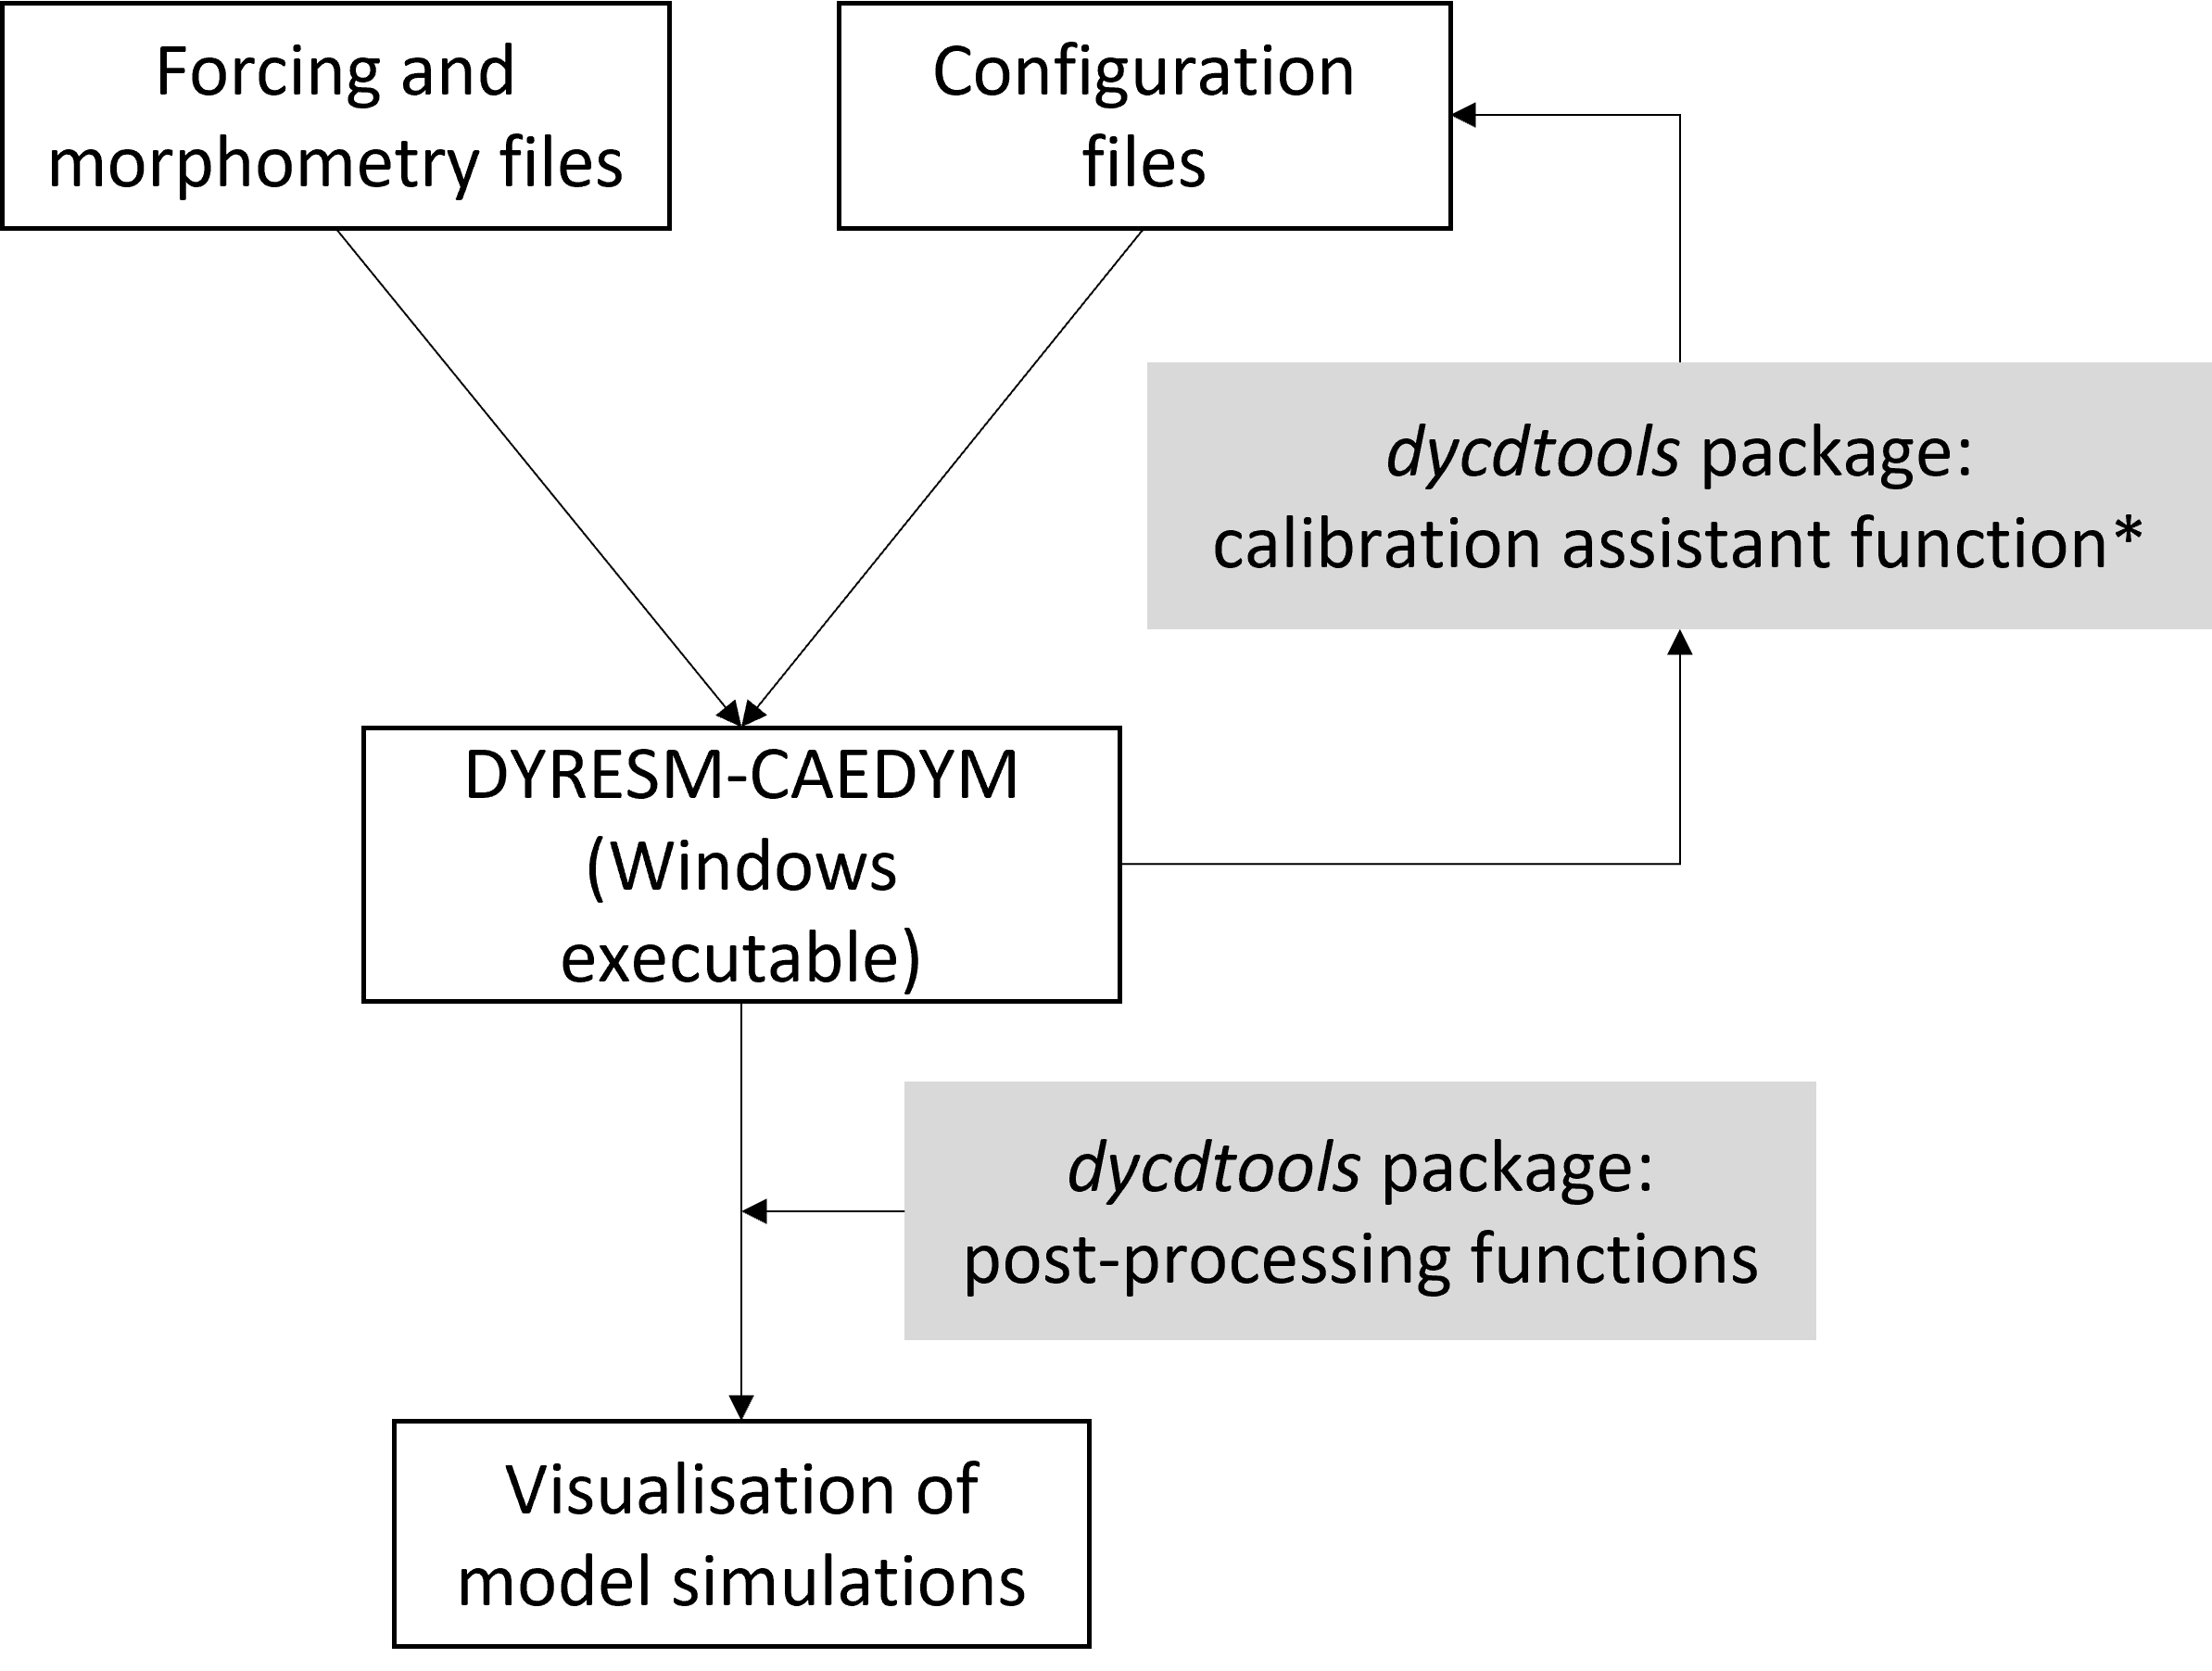
\includegraphics[scale=0.6]{Figure1}
  \caption{DYRESM-CAEDYM simulation process. The calibration assistant function in the \CRANpkg{dycdtools} package deals with the model configuration files (the top shading rectangle), while the post-processing functions can be used to visualise model outputs (the bottom shading rectangle). *The calibration assistant function  works only on the Windows platform, as it needs to call the Windows executable of DYRESM-CAEDYM to run model simulations, while the post-processing functions are cross-platform.}
  \label{figure1}
\end{figure}

\section{Structure of the dycdtools package}

There are two main function categories in the \CRANpkg{dycdtools} package: calibration assistant and post-processing (Table~\ref{Table1}). After the forcing and morphometry input data to DYRESM-CAEDYM have been prepared, the calibration assistant function can be used to 1) choose the optimal set of parameter values for a model simulation application to a lake, or 2) conduct sensitivity analysis of parameters of interest including using a Monte-Carlo parameter perturbation function. Post-processing includes a suite of R functions to visualise DYRESM-CAEDYM output in multiple ways, such as contours, profiles, time series, and scatterplots, for different simulation and observation depths (Table~\ref{Table1}).

\begin{table}[ht]
    \centering
    \caption{List of functions in the dycdtools package for calibration assistant and post-processing and their descriptions.}
    \begin{tabular}{p{0.17\textwidth}p{0.5\textwidth}p{0.23\textwidth}}
    \toprule
    Function name & Description & Categories\\
    \midrule
    calib.assist & Apply different combinations of selected parameter values and output corresponding values of goodness-of-fit by calculating objective functions. Users can choose the optimal set of parameter values or refine potential parameter value ranges based on the calculated values of goodness-of-fit. & calibration assistant\\
    plot\textunderscore cont & Contour plot (heat map) showing a depth- and time-resolved matrix of biogeochemical variables. & post-processing\\
    plot\textunderscore prof & Profile graph of simulations over time (only for dates when observations are available), with variable values shown in the x axis and depth in the y axis. & post-processing\\
    plot\textunderscore ts & Time series plot of simulations for one or multiple specific depths, with time as the x axis and variable values as the y axis. & post-processing\\
    plot\textunderscore scatter & Scatter plot with observations as the x axis and simulations as the y axis. Points in the scatter plot are colour coded by depth. & post-processing\\
    \bottomrule
    \end{tabular}
    \label{Table1}
\end{table}

\subsection{Calibration assistant function}
The calibration assistant function carries out simulations with a large number of possible combinations of parameter values that users regard as potentially suitable for their model calibration, and calculates the values of nominated objective functions (i.e. statistical measures of goodness-of-fit) for each combination. Based on the calculated objective function values, users can determine the optimal set(s) of parameter values or narrow the ranges of possible parameter values. Note that the calibration assistant function does not have the source codes of DYRESM-CAEDYM, but calls the Windows executable of the lake model to run separate simulations with various combinations of parameter values. For this reason, the calibration assistant function can only work on the Windows platform.\par

The calibration assistant function first requires that users prepare a list of sensitive parameters for their simulation (Figure~\ref{figure2}). The selection of sensitive parameters can be made by referring to previous literature \citep{bruce2006numerical,robson2004three,schladow1997prediction} or through expert opinion \citep{lehmann2018modelling} as well as by using a parameter sensitivity analysis, which is a part of the calibration assistant function \citep{ofir2017predicting}. The list of selected sensitive parameters should be prepared as comma-separated values (.csv) in a file input to the function. The potential value range and the preferred number of values within the range for each parameter also need to be defined by users in the csv file. To facilitate this process, an example csv file of many common parameters has been included in the package data set, so that users can follow the given format and adjust values to their specific case study.\par

Based on the user-defined potential value range and the preferred number of values, the calibration assistant function forms all possible combinations of parameter values (Figure~\ref{figure2}). For example, for three parameters that have three different values, there are 3\textsuperscript{3}=27 possible combinations. Users can choose to make the function try every possible combination for model calibration or only a subset of randomly selected combinations. To help users deal with complicated situations where much more parameter combinations are involved, the calibration assistant function is able to parallelise DYRESM-CAEDYM simulations with multiple cores, which could substantially reduce model running time.\par

For each of the combinations, the calibration assistant function makes changes to configuration files and then calls the DYRESM-CAEDYM model to run simulations (Figure~\ref{figure2}). After each model run, the function extracts model outputs to compare against the observations and calculates objective function values. Five commonly used objective functions are currently available in the package: Nash-Sutcliffe Efficiency (NSE) coefficient, Root Mean Square Error (RMSE), Mean Absolute Error (MAE), Relative Absolute Error (RAE), and Pearson’s r (Pearson), with more to be added in an update of the package by referring to the inventory of different statistical measures in \citet{bennett2013characterising}. The output of the calibration assistant function is a table that outlines all combinations of parameters that were used and the corresponding objective function values. Based on the output, users can determine the optimal set(s) of parameter values (e.g., the set that gives the highest NSE value or highest weighted average values for NSE and RMSE) or narrow the range of suitable parameter values.\par

\begin{figure}[ht]
    \centering
    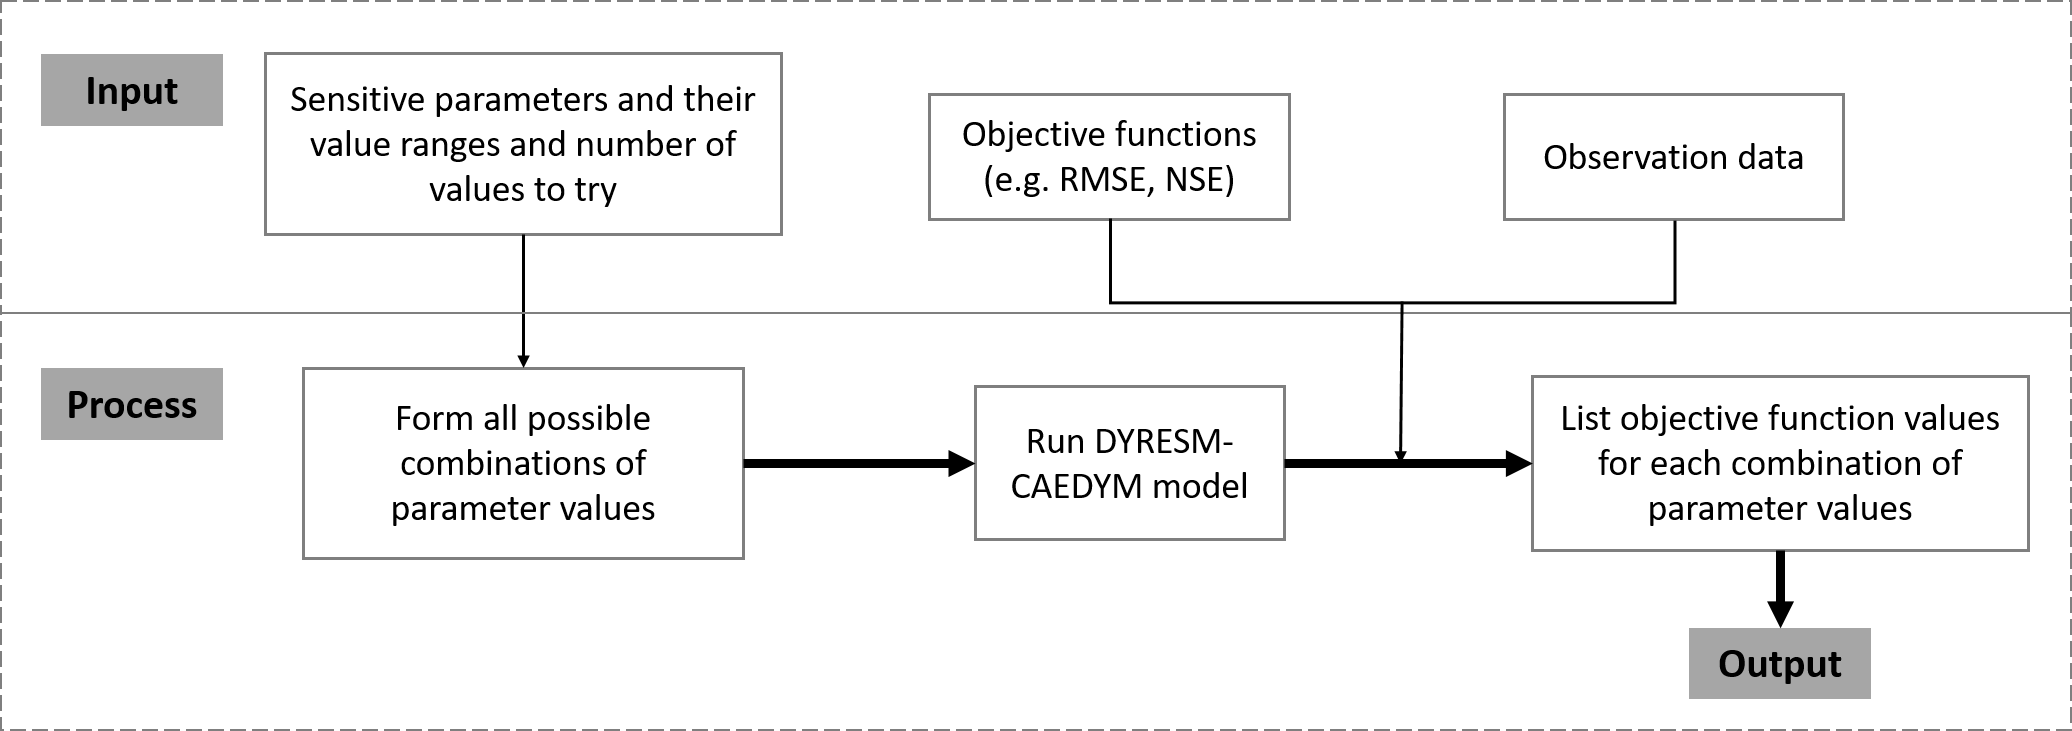
\includegraphics[scale = 0.39]{Figure2}
    \caption{Structure of the calibration assistant function. Three key inputs to the calibration assistant function include a list of sensitive parameters and their assigned value ranges, objective functions, and observation data. The function forms scenarios, runs DYRESM-CAEDYM model on each of the scenarios, and outputs objective function values.}
    \label{figure2}
\end{figure}

The calibration assistant function can also be used for parameter sensitivity analysis by automatically modifying parameter values. Two commonly used methods for sensitivity analysis, One At a Time (OAT) and All At a Time (AAT), can be carried out through this function by setting the “combination” argument as “all” and preparing specifically designed parameter combinations. An OAT analysis changes a single parameter at a time and is suitable for local sensitivity analysis, while ATT modifies multiple parameters simultaneously and is suitable for global sensitivity analysis, notably when there are nonlinear relationships between parameter and model outputs. Increasing numbers of environmental modelling studies report model uncertainty for a variety of purposes, including assessment of model errors, model calibration communication and diagnostic evaluation \citep{couture2018simulating,dietzel2014bayesian,pianosi2016sensitivity}. This function is also flexible, allowing users to try a subset of randomly selected parameter combinations (e.g. Monte-Carlo parameter perturbation) or a carefully selected combination by setting the “combination” argument as “random”.\par

\subsection{Post-processing functions}

Post-processing functions provide multiple ways to visualise DYRESM-CAEDYM outputs, as follows:

\begin{itemize}
    \item Function “plot\textunderscore{}cont” displays a heat map of variable values with depth within the water column and over time. This visualisation is particularly suitable for displaying temporal and depth dynamics of a variable at one lake site.
    \item Function “plot\textunderscore{}prof” shows vertical profiles of the simulation and corresponding observations, for all dates where observations are available.
    \item Function “plot\textunderscore{}ts” plots simulated values and observations for a specified variable and depth over time. It can be used to compare temporal changes of a variable for simulations and observations at specific depths.
    \item Function “plot\textunderscore{}scatter” shows observations against simulated values for corresponding time and depth, with a colour scale representing measured depth. It can be used to demonstrate visually the goodness of fit for a variable across the water column.
\end{itemize}

All four types of graphs can be used to compare simulations and observations in the same figure. Examples of each type of graph are shown in the following section.

\section{Minimal case study example}
Lake Okareka is a medium size lake in the Bay of Plenty region of North Island, New Zealand. It has a surface area of 3.46 km\textsuperscript{2}, a land catchment area of 16.7 km\textsuperscript{2} and a maximum depth of 33.5 meters. Water drains from the lake via an outlet canal towards a large downstream lake, Tarawera. The \CRANpkg{dycdtools} package was used to calibrate three parameters for the lake temperature simulation and visualise the temperature simulation against observed data with the four aforementioned plotting functions. The three calibrated parameters were wind stirring efficiency, vertical mixing coefficient, and light extinction coefficient, as they have been found to be most sensitive in temperature simulations in other lake systems \citep{weinberger2012using}. \par

The simulations were conducted with forcing inputs (e.g., meteorology, inflows and outflow) at a daily time step over the period of 2002-01-23 to 2016-12-31. The meteorology and outflow data were respectively collected from the New Zealand National Climate Database (\url{https://cliflo.niwa.co.nz}) and an environmental monitoring website (\url{https://www.boprc.govt.nz/environment/maps-and-data/environmental-data}). Discharge output from a SWAT model application (unpublished) was used as catchment surface inflow to the lake. All example data are provided in a public data repository (\url{https://doi.org/10.5281/zenodo.7431128}) for users to familiarise themselves with model runs, calibration and visualisation. \par

The calibration assistant function deals with the configuration files. In this simulation, both the wind stirring efficiency and vertical mixing coefficient are in the parameter (.par) file, while the light extinction coefficient is in the configuration (.cfg) file. We assigned a range and a preferred number of values to try for each of the three parameters to form a sequence of possible values (Table~\ref{table2}). 

\begin{table}[htbp]
    \centering
    \caption{Three parameters that were calibrated with assigned value ranges and preferred number of values to try (N\textunderscore values). The columns of “Input file” and “Line No.” describe the line of the input file where the parameter is located.}
    \begin{tabular}{c c c c c c c }
    \toprule
    Parameter & Unit & Min & Max & N\textunderscore{}values & Input file & Line No.\\
    \midrule
    Wind stirring efficiency & - & 0.2 & 0.8 & 4 & Okareka.par & 12\\
    Vertical mixing coefficient & - & 100 & 700 & 4 & Okareka.par & 15\\
    Light extinction coefficient & m\textsuperscript{-1} & 0.1 & 0.25 & 4 & Okareka.cfg & 7\\
    \bottomrule
    \end{tabular}
    \label{table2}
\end{table}

The calibration assistant function tried all combinations of the three parameter values and calculated the objective function NSE for each model run. We chose the combination of parameter values that gave the highest NSE values as the optimal set and then used the post-processing tools to plot simulations against observations in four different ways. The R code for using the calibration assistant function in this example is as follows:

\begin{example}
   # Assisting calibration of DYRESM-CAEDYM using the dycdtools package
    library(dycdtools)
    calib.assist(cal.para = "calibration_data/Calibration_parameters.csv",
                 combination = "all",
                 model.var = "TEMP",
                 obs.data = "calibration_data/Obs_data_template.csv",
                 objective.function = "NSE",
                 start.date = "2002-01-23",
                 end.date = "2016-12-31",
                 dycd.wd = "calibration_data/DYRESM_CAEDYM_Lake-Okareka/",
                 dycd.output = "calibration_data/DYRESM_CAEDYM_Lake-Okareka/DYsim.nc",
                 file.name = "calibration_data/Calibration_outputs.csv",
                 write.out = TRUE,
                 parallel = TRUE,
                 verbose = TRUE)
\end{example}

Given each parameter had four assigned values, the calibration assistant function called DYRESM-CAEDYM to run a total of 4\textsuperscript{3} = 64 combinations for the three parameters. For each model run, the objective function NSE was calculated for temperature simulations. A heat map is a good way to visualise the variations in these NSE values under different combinations of parameter values. An example of R code for producing a heat map of the auto-calibration outcome is as follows:

\begin{example}
    # Read in model calibration results
    calibration <- read.csv("calibration_data/Calibration_outputs.csv")

    # Heat map
    library(ggplot2)
    ggplot(calibration, aes(x = wse,y = vmc,fill = NSE.TEMP)) +
           geom_tile() +
           scale_fill_distiller(palette = "PuBu", direction = 1) +
           facet_grid(~lec, scales = "free") +
           xlab("Wind stirring efficiency") +
           ylab("Vertical mixing coefficient") +
           labs(title = "Light extinction coefficient", fill = "NSE") +
           theme_bw()  +
           theme(plot.title = element_text(size = 11, hjust = 0.5))
           
    ggsave(filename = "Figure_03.png", width = 8, height = 4)
\end{example}

The calculated NSE values varied significantly among the combinations, ranging from 0.03 to 0.95. The combination of wind stirring efficiency = 0.6, vertical mixing coefficient = 500, and light extinction coefficient = 0.25 m\textsuperscript{-1} achieved the highest NSE value of 0.95 (i.e., considered to be the optimal set of parameter values) (Figure~\ref{figure3}). 

\begin{figure}[ht]
    \centering
    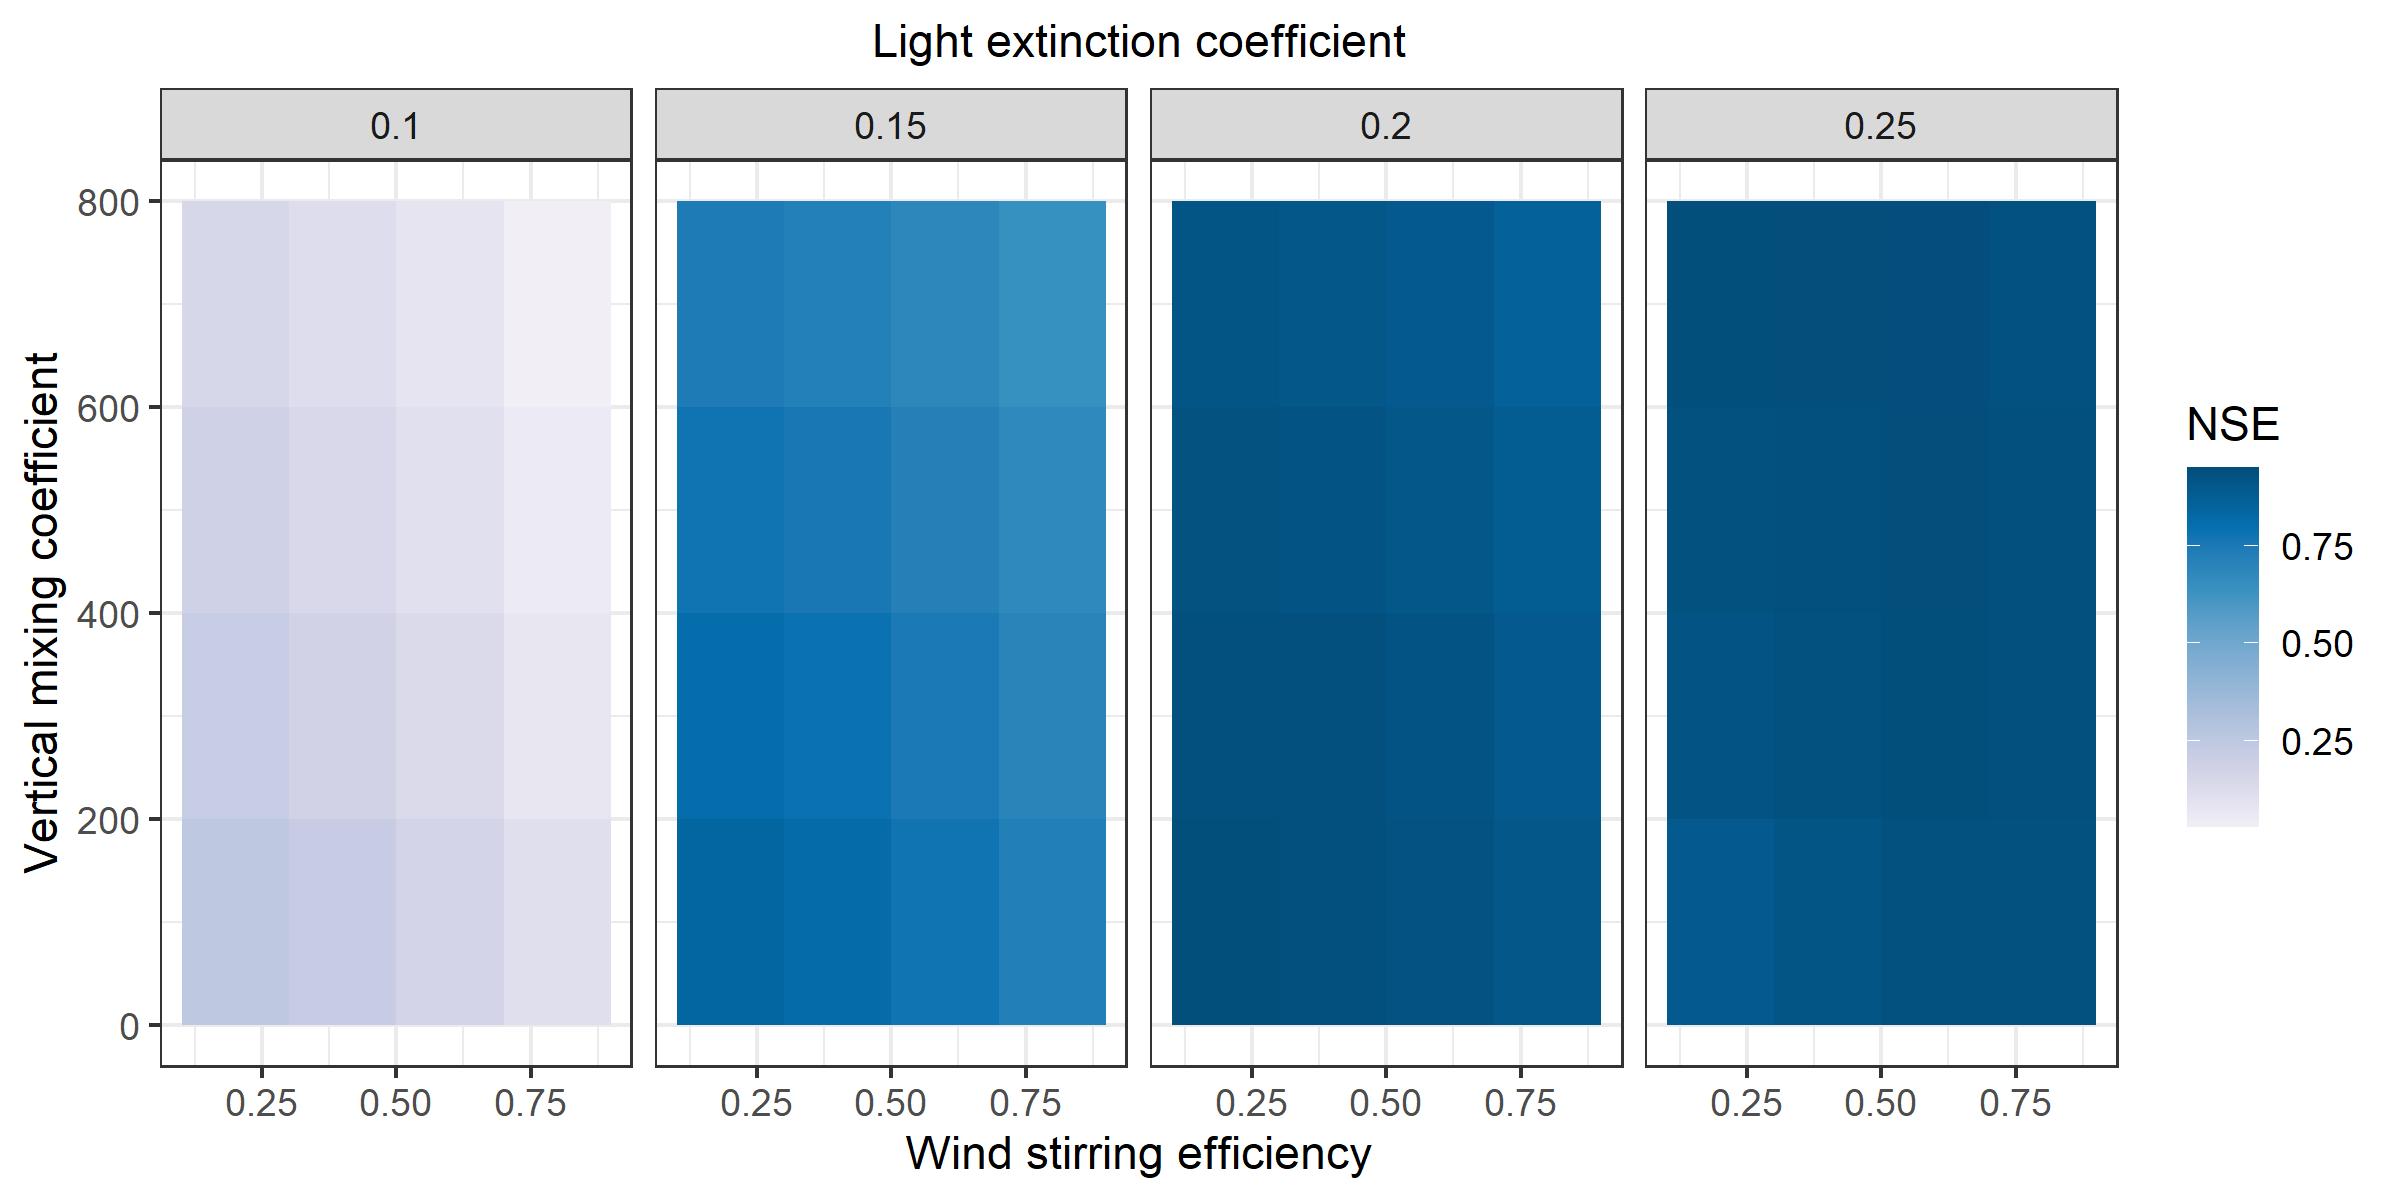
\includegraphics[scale = 0.62]{Figure3}
    \caption{Heat map of Nash-Sutcliffe Efficiency (NSE) coefficient values for temperature simulations in Lake Okareka estimated for the combinations of three parameters given in Table~\ref{table2} (wind stirring efficiency, vertical mixing coefficient, and light extinction coefficient [m\textsuperscript{-1}]). The darker the colour, the better the model performance (measured as NSE).}
    \label{figure3}
\end{figure}

A few other combinations could also achieve similar outcomes. For example, when the light extinction coefficient = 0.25 m\textsuperscript{-1}, the NSE values ranged between 0.90 and 0.95, regardless of the wind stirring efficiency and vertical mixing coefficient values shown in Table 2. Figure 3 also revealed that temperature simulations were generally poor when light extinction coefficient = 0.1 and 0.15 m\textsuperscript{-1}, suggesting that these values of light extinction coefficient are too low to achieve a suitably accurate temperature simulation for Lake Okareka.\par

Under the optimal set of parameter values identified from the calibration assistant function (Figure~\ref{figure3}), we re-ran the DYRESM-CAEDYM model and visualised the temperature simulations with the four post-processing functions. An example R code for visualisation functions is shown preceding the corresponding figure.\par

The temperature simulations in Lake Okareka displayed a clear and consistent seasonal pattern. Temperature was up to 24 °C in the summer season and was below 10 °C in the winter (Figure~\ref{figure4}). The simulation contour plot showed that the thermocline of Lake Okareka (the layer of most rapid temperature change) was around 15 m in summer, but the lake always mixed in winter (Figure~\ref{figure4}), corresponding to isothermal conditions over the water depth, suggesting a monomictic lake mixing regime. Observations are shown as dots in Figure~\ref{figure4} and match well with simulations both spatially (i.e., vertically) and temporally (i.e., horizontally).\par

\begin{example}
    # Extract temperature simulations
    var.values <- ext_output(dycd.output = "DYCD_Okareka/DYsim.nc",
                             var.extract = c("TEMP"))

    # Interpolation of temperature across water column at an interval of 0.5 m
    temp.interpolated < -interpol(layerHeights = var.values$dyresmLAYER_HTS_Var,
                                  var = var.values$dyresmTEMPTURE_Var,
                                  min.dept = 0, max.dept = 33, by.value = 0.5)

    # Read in observed water quality data
    obs.okareka <- read.csv("plotting_data/Obs_data_template.csv")
    obs.okareka$Date <- as.Date(obs.okareka$Date,format="%d/%m/%Y")
    # subset observed data to remain temperature observations
    obs.temp <- obs.okareka[, c('Date','Depth','TEMP')] 

    # Contour plot
    png(filename = 'Figure_04.png', width = 1200, height = 700)
    plot_cont_com(sim = temp.interpolated,
                  obs = obs.temp,
                  plot.start = "2002-01-23",
                  plot.end = "2006-12-31",
                  sim.start = "2002-01-23",
                  sim.end = "2016-12-31"
                  legend.title = "T\n(\u00B0C)",
                  min.depth = 0,
                  max.depth = 33,
                  by.value = 0.5,
                  nlevels = 20)
    dev.off()
\end{example}

\begin{figure}[htbp]
    \centering
    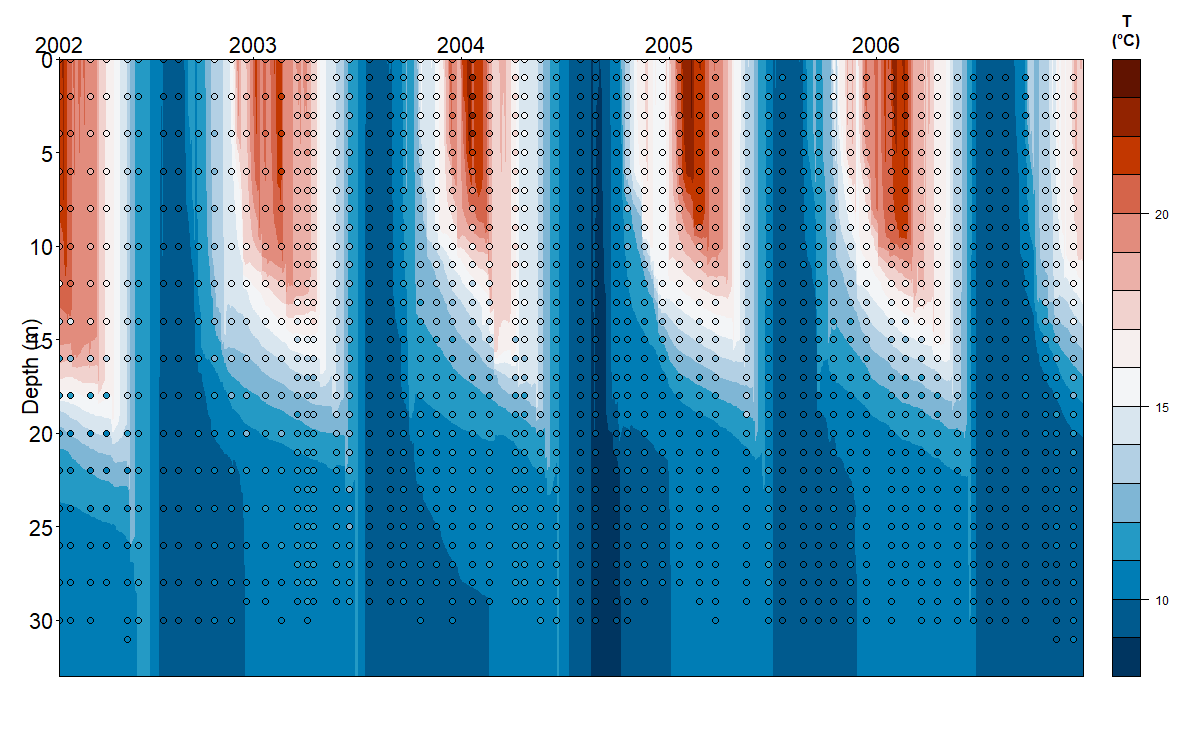
\includegraphics[scale=0.33]{Figure4.png}
    \caption{Example contour plot of temperature simulations and observations for Lake Okareka from 2002-01-23 to 2006-12-31. Each dot represents an observation at a specific depth on a specific date. Dots are colour coded on the same scale (right-hand side) as the simulation.}
    \label{figure4}
\end{figure}

\newpage

Simulations and observations of temperature with depth are shown in Figure~\ref{figure5} for the dates when observations were available. The vertical profiles provide a more discerning view of details such as the thermocline depth in Lake Okareka. The simulated temperature profile mostly aligned well with the observed profile but had a tendency to overestimate the depth of the thermocline in the first summer (early 2002), whilst capturing the timing of mixing (little or no temperature gradient) in winter.\par

\begin{example}
    # Profile plot
    plot_prof(sim = temp.interpolated,
              obs = obs.temp,
              sim.start = "2002-01-23",
              sim.end = "2016-12-31",
              plot.start = "2002-01-23",
              plot.end = "2002-12-31",
              min.depth = 0,
              max.depth = 33,
              by.value = 0.5,
              xlabel = "Temperature \u00B0C")
              
   ggsave(filename = "Figrue_05.png", height = 4, width = 7)

\end{example}

\begin{figure}[htbp]
    \centering
    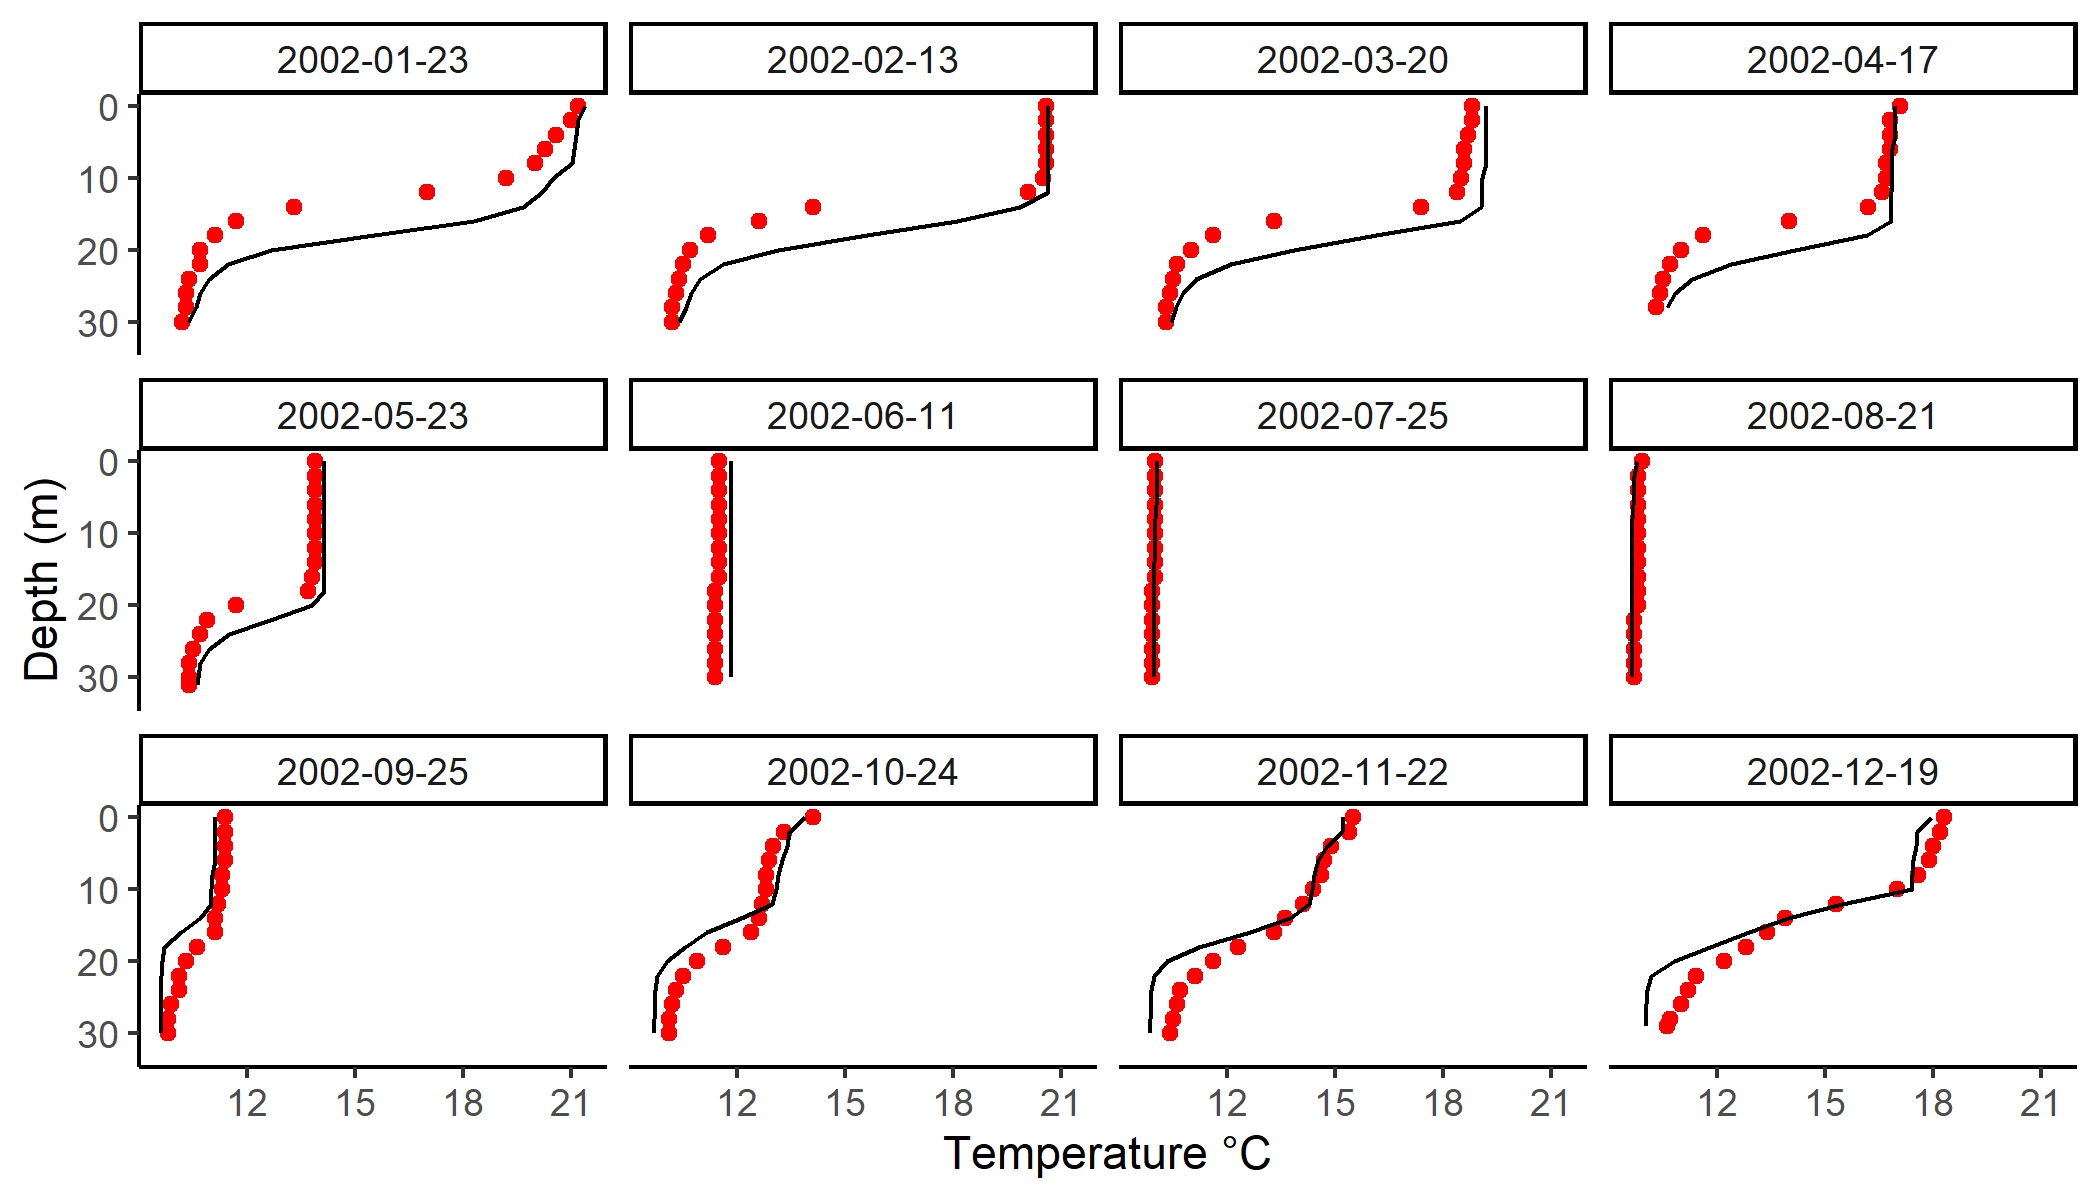
\includegraphics[scale=0.78]{Figure5.png}
    \caption{Example profile plots of temperature simulations (black line) and observations (brown dots) for Lake Okareka from 2002-01-23 to 2002-12-19, available for each observation occasion. The profile plots shows a seasonable pattern of stratification and mixing in the lake over the 12 months time, and the model was able to repeat the pattern.}
    \label{figure5}
\end{figure}

\newpage

The time series figure displays temperature simulations as a continuous line for a specific depth over the entire simulation period, with observations shown as dots (Figure~\ref{figure6}). The temperature in the surface of the lake (1 m deep) varied strongly over the years, with a clear seasonal pattern, while at mid-depth (14 m deep) it varied to a lesser degree but showed a similar pattern, and in the near-bottom (30 m deep) layer it remained relatively unchanged.\par

\begin{example}
    # Time series plot
    p <- plot_ts(sim = temp.interpolated,
                 obs = obs.temp,
                 target.depth = c(1, 14, 30),
                 sim.start = "2002-01-23",
                 sim.end = "2016-12-31",
                 plot.start = "2002-01-23",
                 plot.end = "2012-12-31",
                 min.depth = 0,
                 max.depth = 33,
                 by.value = 0.5,
                 ylabel = "Temperature \u00B0C")
                 
    rmse_dpt01 <- objective_fun(sim = temp.interpolated[2:4,],
                                obs = obs.temp[obs.temp$Depth == 1, ],
                                fun = c('RMSE'),
                                start.date = '2002-01-23',
                                end.date = '2016-12-31',
                                min.depth = 0.5,
                                max.depth = 1.5,
                                by.value = 0.5)

   rmse_dpt14 <- objective_fun(sim = temp.interpolated[28:30,],
                              obs = obs.temp[obs.temp$Depth == 14, ],
                              fun = c('RMSE'),
                              start.date = '2002-01-23',
                              end.date = '2016-12-31',
                              min.depth = 13.5,
                              max.depth = 14.5,
                              by.value = 0.5)
                              
\end{example}

\newpage

\begin{example}
   rmse_dpt30 <- objective_fun(sim = temp.interpolated[60:62,],
                              obs = obs.temp[obs.temp$Depth == 30, ],
                              fun = c('RMSE'),
                              start.date = '2002-01-23',
                              end.date = '2016-12-31',
                              min.depth = 29.5,
                              max.depth = 30.5,
                              by.value = 0.5)

   rmse_text <- data.frame(x = as.Date('2007-06-01'),
                           y = 25,
                           Depth = c(1, 14, 30),
                           label = c(paste0('RMSE = ', round(rmse_dpt01$RMSE,2), ' \u00B0C'), 
                                     paste0('RMSE = ', round(rmse_dpt14$RMSE,2), ' \u00B0C'), 
                                     paste0('RMSE = ', round(rmse_dpt30$RMSE,2), ' \u00B0C')))

   p + ylim(8,26) +
       geom_text(data = rmse_text, 
                 mapping = aes(x = x, y = y, label = label))
            
   ggsave(filename = 'Figure_06.png', height = 4, width = 7)

\end{example}

\begin{figure}[htbp]
    \centering
    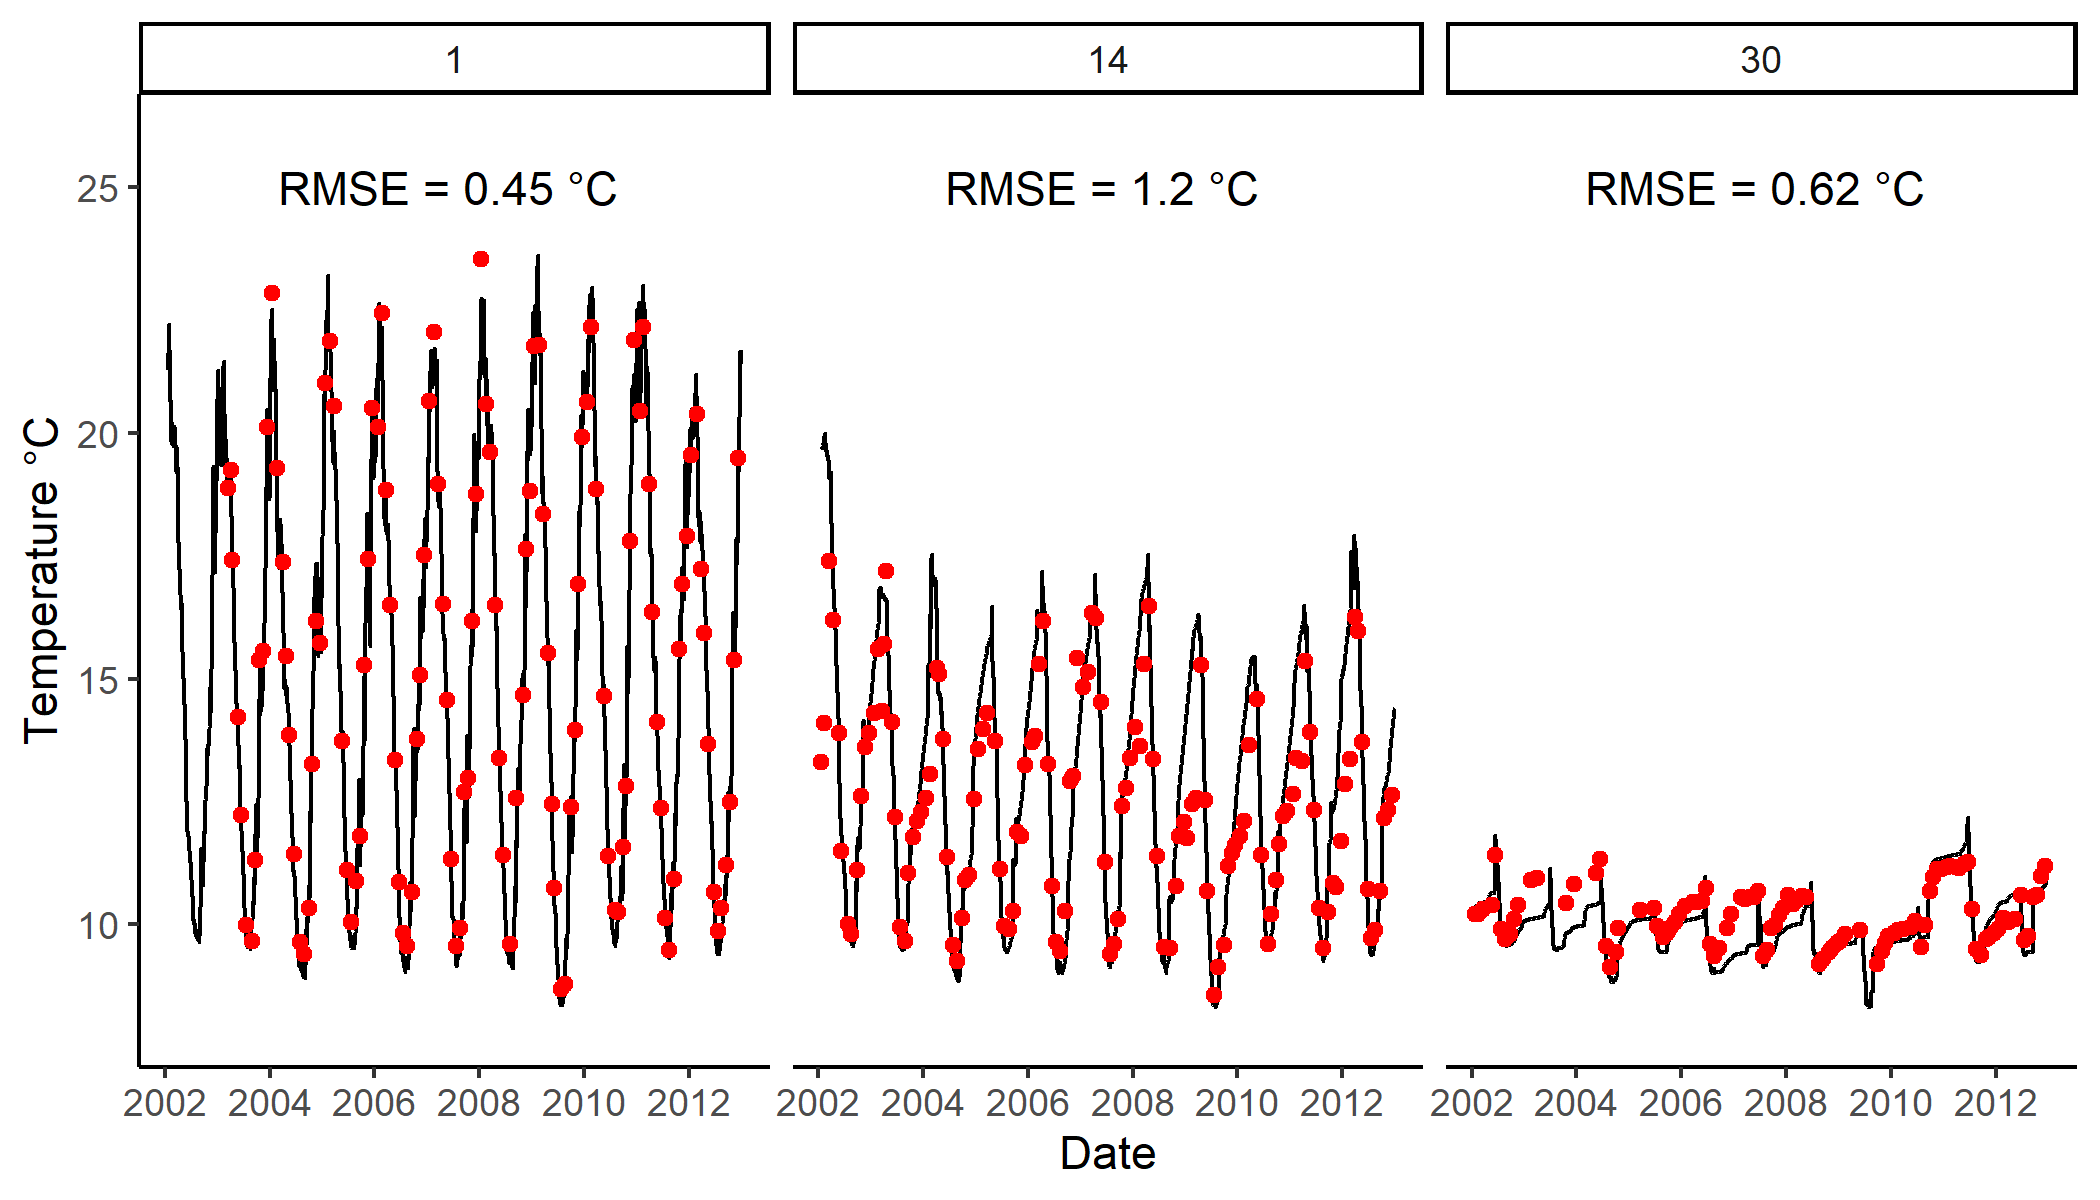
\includegraphics[scale=0.78]{Figure6.png}
    \caption{Example time series plot of temperature simulations (black line) and measurements (brown dots) for three depths (upper row box; 1 m – near-surface layer, 14 m – middle layer close to the thermocline, and 30 m – near-bottom layer) of Lake Okareka from 2002-01-23 to 2012-12-31. The RMSE values calculated from the 'objective\_fun' function in the package are also shown for each depth profile.}
    \label{figure6}
\end{figure}

The scatter plot compares all temperature simulation values against observations denoted as dots in a Cartesian coordinate system, with a reference line of y=x to indicate the ideal fit (1:1) of simulations to observations. Each point is colour coded by depth. The majority of dots were close to the reference line, indicating good performance of DYRESM-CAEDYM in the temperature simulation (Figure~\ref{figure7}).\par

\newpage

\begin{example}
    # Scatter plot
    plot_scatter(sim=temp.interpolated,
                 obs=obs.temp,
                 sim.start="2002-01-23",
                 sim.end="2016-12-31",
                 plot.start = "2002-01-23",
                 plot.end="2012-12-31",
                 min.depth = 0,
                 max.depth = 33,
                 by.value = 0.5)
                 
    ggsave(filename = 'Figure_07.png', height = 4, width = 7)
\end{example}

\begin{figure}[htbp]
    \centering
    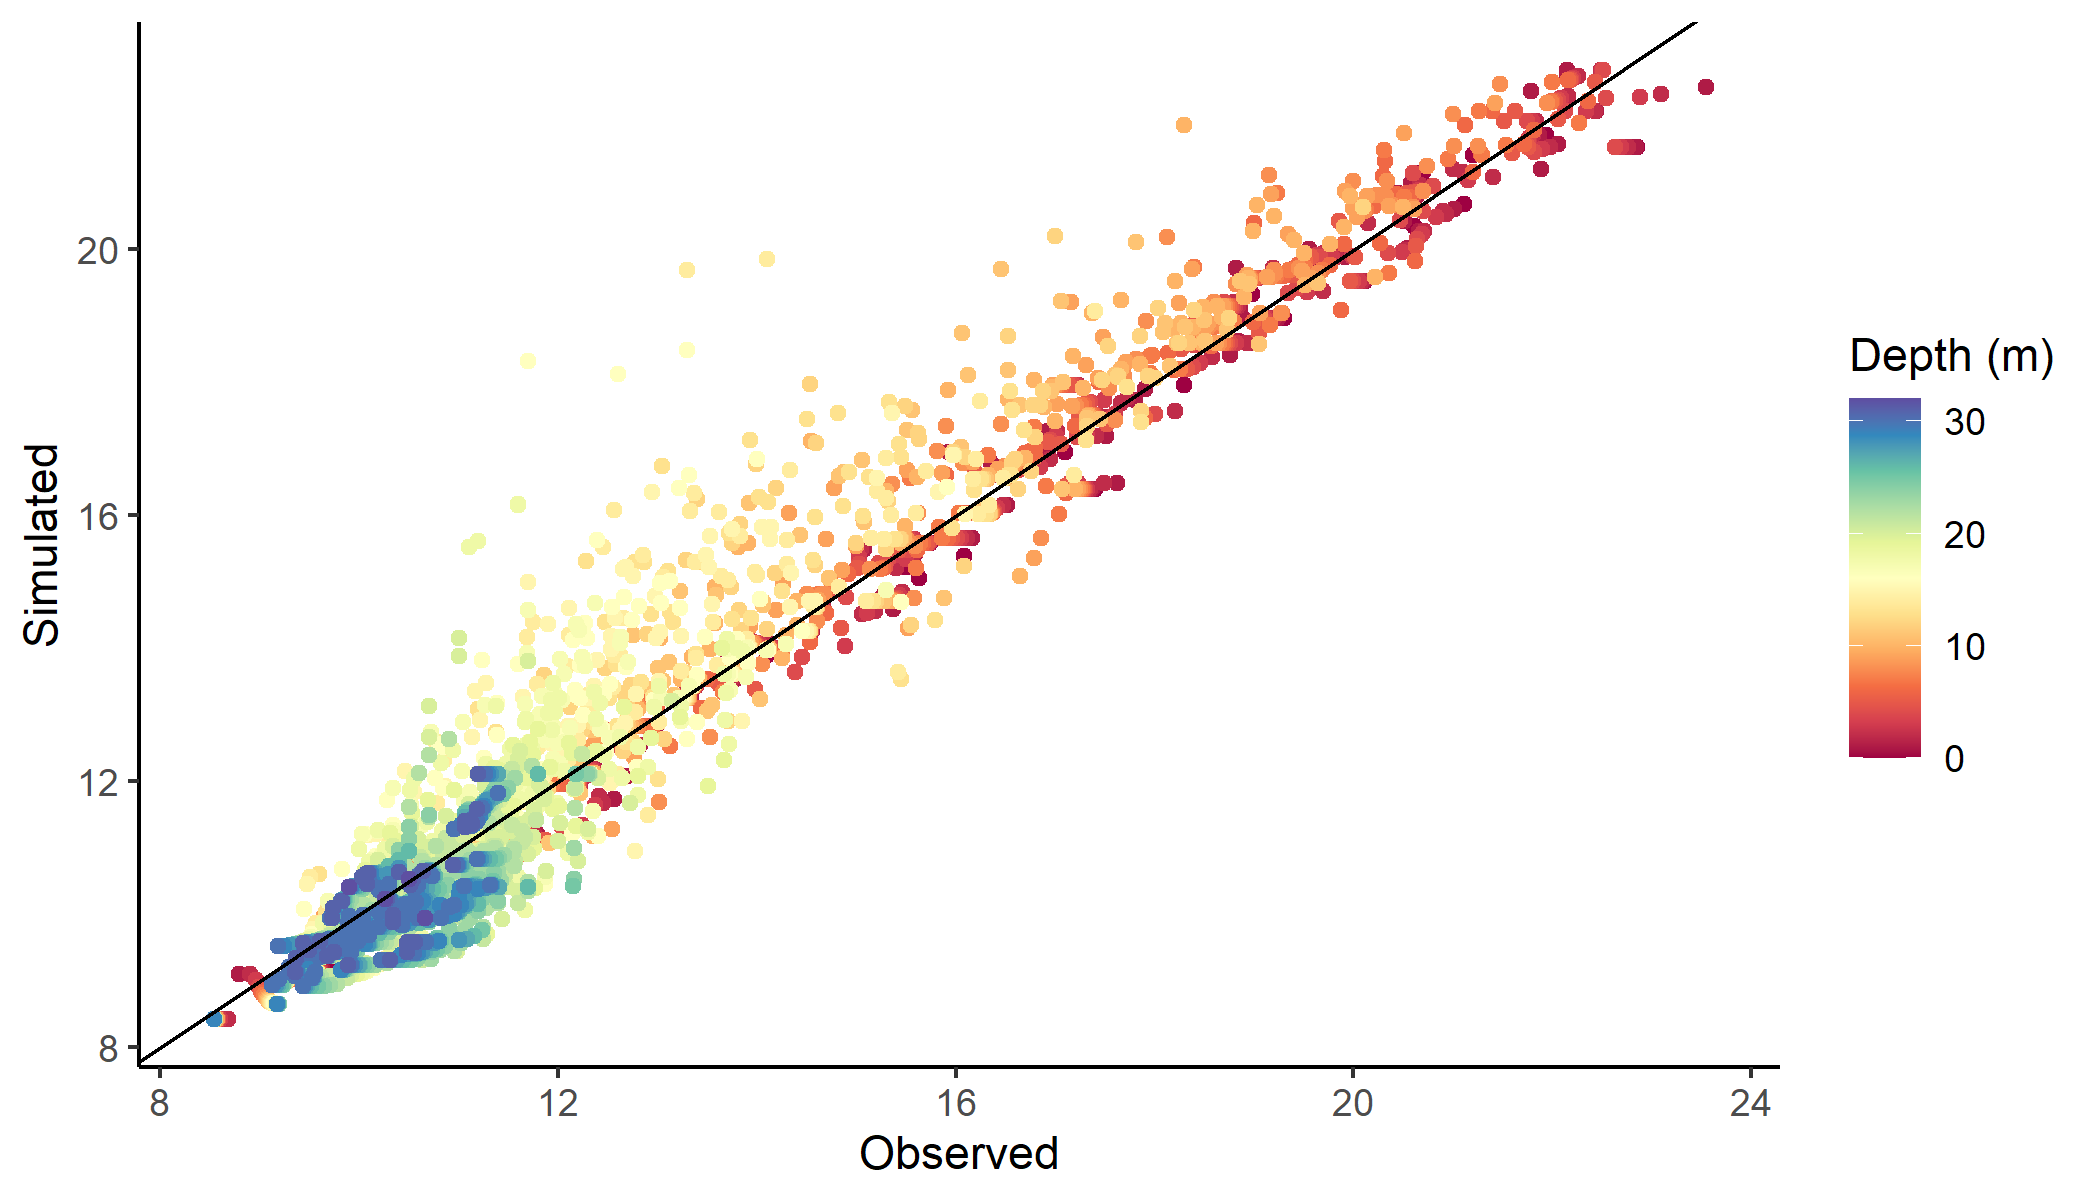
\includegraphics[scale=0.78]{Figure7.png}
    \caption{Example scatterplot of temperature simulations and observations for Lake Okareka from 2002-01-23 to 2012-12-31. Note that the dots are colour coded by depth. The red line is a 1:1 slope, i.e., simulated temperature = observed temperature. The plot indicates a good model performance as the majority of the dots are located around the black line.}
    \label{figure7}
\end{figure}

\section{Discussion}

Aquatic ecosystem models have increasingly been used to shed light on lake ecosystem function \citep{scheffer2001catastrophic} and inform policy and management decisions to improve water quality and control eutrophication \citep{wang2012flickering}. With progressive increases in the number and complexity of processes represented, and increasing computational power, these models have increased in complexity and have a large number of parameters. These types of models generally require extensive calibration to be suitable for lake-specific simulations, which is quite challenging, despite the development of parameter priors libraries \citep{robson2018towards} that can help with understanding possible ranges of parameters and synthesise values used in other studies. In addition, multifaceted and multi-layered modelling results need to be visualised in various ways to express model uncertainty and communicate effectively with a broader community that may be engaged in understanding and interpreting the implications of model scenarios. Here, we have presented an open-source R package \CRANpkg{dycdtools} to help address these challenges in calibrating a widely used aquatic ecosystem model DYRESM-CAEDYM and visualising its simulation results. Importantly, this package has the potential to be adjusted for other aquatic ecological models with a similar structure.\par

\subsection{Calibration assistant function}

The output of the calibration assistant function in the \CRANpkg{dycdtools} package is a list of combinations of parameter values with their objective function values, rather than a single optimal set of parameter values provided by many auto-calibration algorithms, such as the auto-calibration module in the RAPID model developed in \citet{david2011river}, the auto-calibration algorithm proposed in \citet{luo2018autocalibration}, and the Genetic Algorithm developed in \citet{goldberg1988genetic}. We chose not to provide a single parameter set partly due to the potential for parameter equifinality \citep{beven1992future}, a classical problem of optimisation where different sets of parameter values may provide similar simulation fit to observations. This problem is particularly pertinent for complex aquatic ecosystem models (e.g., DYRESM-CAEDYM) that include a large number of parameters. Many studies illustrated the difficulties of finding a single optimal set of parameter values in the high-dimensional parameter space, due to inter-correlation between parameters and autocorrelation of the residuals \citep{fernandez2010optimal,gupta2006model}. Therefore, instead of using an auto-calibration algorithm to decide the optimal set of parameter values, we suggest users compare those combinations of parameter values that result in high objective values and manually choose the combination that they believe is the most physically meaningful. Such a process aligns with the concept of development of user expertise and knowledge that are critical for successful model applications \citep{hipsey2015predicting}.\par

It is worth noting that an objective function is a means to characterise the performance of environmental models, and is useful and often necessary \citep{bennett2013characterising}. A substantial body of work has been done to propose methods and criteria to judge the performance of environmental models, often for hydrological models \citep{jakeman2006ten,krause2005comparison} and less frequently for ecological models \citep{risbey1996assessing}. Many of the proposed objective functions have been summarised in \citet{bennett2013characterising} and can be applied to characterise performance of lake models. Five of the most commonly used objective functions have been included in the current package, and we plan to add functions to give users more choices of characterising model performance and to better inform parameter calibration.\par

Given that it is not realistic to expect any one set of parameter values to be truly representative of the actual parameter set \citep{beven1992future}, it is also important to convey the accuracy of the simulations and the associated uncertainties. In lake modelling, multi-parameter perturbation has been conducted using Monte-Carlo techniques to inform parameter uncertainty effects \citep{luo2018autocalibration,muraoka2019novel}. The calibration assistant function developed here can be used to carry out such a sensitivity analysis by perturbing multiple parameters within a certain range when the “combination” argument is set to “random”. User expert knowledge \citep{lehmann2018modelling} and parameter priors libraries \citep{robson2018towards} are also valuable in narrowing parameter ranges which can be important in reducing computation times of calibration and sensitivity analysis, as well as reducing the incidence of common issues such as equifinality.\par

\subsection{Suggestions on the use of calibration assistant function}

The calibration assistant function developed in this study is not intended to replace manual calibration, rather, it is aimed to save time assigned to calibration and sensitivity analysis by automatically trialling a number of parameter values so as to bring a focus to the range of sensitive parameter values. We recommend manual calibration as a means to develop expert knowledge about model parameter values, in an iterative procedure that includes assistant calibration and sensitivity analysis, as well as literature review of parameters. We also recommend a combination of OAT and AAT calibration, with the former used to better understand individual responses of parameters and the latter used with care because exponentially large numbers of possible parameter value combinations are possible and computational times could become untenable even with parallel processing enabled. For example, in the case of 10 parameters where each parameter has three possible values, the total number of possible combinations is 3\textsuperscript{10} = 59,049. If each model run takes 2 minutes, then it would take 59,049 × 2 = 118,098 minutes (> 32 days) to run these combinations.\par

Manual calibration has also been used as a way to work around the difficulties with weighting and prioritising state variables using an auto-calibration procedure \citep{lehmann2018modelling}. Therefore, while acknowledging the benefits of assistant calibration in trialling a number of parameter values without the heavy time burden of manual adjustment, we encourage users to actively engage in the calibration process. More specifically, users may first define suitable value ranges of various parameters from the literature (including other modelling studies) and lab or field experiments \citep{robson2018towards}, and then conduct both manual and automated sensitivity analysis to understand which parameters are sensitive and should be more strategically evaluated. Finally, users can apply both the calibration assistant function and manual calibration to optimise parameter values. This process can be repeated multiple times until users are satisfied with accuracy of the simulations, assessed using quantitative output statistics and qualitative comparisons with observed data.\par

\subsection{Visualisation of model outputs}

Visualisation of model outputs is an important tool for effectively engaging academic, the public and environmental managers in expressing model uncertainty, and as a prerequisite for improving confidence in scenario simulations. This is particularly true for multidimensional model outputs that are intangible, and visualisation has a fundamental role in exploring information and generating understanding \citep{mcinerny2014information}. The \CRANpkg{dycdtools} package expands on existing lake model visualisation tools, such as contours, profiles and time series used by the \CRANpkg{glmtools} and \pkg{LakeEnsemblR} packages, by providing additional functionality including scatterplots. Each of the plotting functions is designed to best suit different presentation purposes, as outlines in the "Post-processing functions" Section. We anticipate that the developed visualisation tools in \CRANpkg{dycdtools} package can not only complement the existing associated GUI by providing more flexible ways of visualising DYRESM-CAEDYM model outputs, but can also be adapted for other lake ecosystem models, such as the General Lake Model \citep{hipsey2019general} and the Fresh-water Lake Model for LM \citep{Mironov2010ImplementationOT}.\par

In summary, dycdtools is a modular, flexible, and open-source tool that is designed to make the calibration process of the DYRESM-CAEDYM model substantially less time-consuming and to visualise complex modelling results in multiple ways for effective communication. It is suitable for users with various levels of expertise. This study places great emphasis on tools to evaluate the quality of model calibration as many of these models need to provide robust simulations that form the basis of scenario simulations, often designed to evaluate different management and environmental (e.g., climate change, land use change) scenarios.\par

\section{Acknowledgements}

We thank Gebiaw Ayele from Australian Rivers Institute, Griffith University for providing the catchment inflow simulations as part of the example data for the DYRESM-CAEDYM model application. We acknowledge Bay of Plenty Regional Council for provision of data for model runs. Author contributions: S.Y., M.F., and C.M. developed the source codes for the R package; S.Y. prepared the application example; and S.Y., D.H., C.M. and M.F. wrote the paper. This research did not receive any specific grant from funding agencies in the public, commercial, or not-for-profit sectors.\par

\section{Data and software availability}

The published dycdtools package can be downloaded from CRAN and the developer version is available from \url{ https://github.com/SongyanYu/dycdtools}. Issues regarding the package can be submitted via \url{https://github.com/SongyanYu/dycdtools/issues}. The executables of DYRESM-CAEDYM and the example data  supporting the case study can be found from \url{https://doi.org/10.5281/zenodo.7431128}. The source codes of DYRESM-CAEDYM are accessible from \url{https://github.com/AquaticEcoDynamics/dy-cd}\par

\bibliography{Yu_dycdtools.bib}

\address{Songyan Yu\\
  Griffith University\\
  Australian Rivers Institute and School of Environment and Science\\
  Australia\\
  ORCID: 0000-0001-5765-7060\\
  \email{sunny.yu@griffith.edu.au}}

\address{Christopher G. McBride\\
  University of Waikato\\
  Environmental Research Institute\\
  New Zealand\\
  ORCID: 0000-0001-5784-9767\\
  \email{cmcbride@waikato.ac.nz}}

\address{Marieke A. Frassl\\
  Griffith University\\
  Australian Rivers Institute and School of Environment and Science\\
  Australia\\
  ORCID: 0000-0001-8843-8477\\
  \email{marieke.frassl@gmail.com}}
  
\address{Matthew R. Hipsey\\
 The University of Western Australia\\
 Aquatic Ecodynamics, UWA School of Agriculture and Environment\\
 Australia\\
 ORCID: 0000-0001-8386-4354\\
 \email{matt.hipsey@uwa.edu.au}}
  
\address{David P. Hamilton\\
  Griffith University\\
  Australian Rivers Institute and School of Environment and Science\\
  Australia\\
  ORCID: 0000-0002-9341-8777\\
  \email{david.p.hamilton@griffith.edu.au}}
